% Activate the following line by filling in the right side. If for example the name of the root file is Main.tex, write
% "...root = Main.tex" if the chapter file is in the same directory, and "...root = ../Main.tex" if the chapter is in a subdirectory.
 
%!TEX root = phys-notes.tex

\section{Motion}

\subsection{Definitions}

Kinematics is the study of motion. It refers only the motion of objects and the positions, without considering their masses or forces.

\begin{definition}
	Displacement is the distance moved in a particular direction from a reference point. It is a vector quantity.
\end{definition}

\begin{definition}
	Velocity is displacement per unit time. It is the first derivative of displacement with respect to time ($\frac{ds}{dt}$), and is a vector quantity.
\end{definition}

\begin{definition}
	Acceleration is change in velocity per unit time. It is the second derivative of displacement w.r.t. time ($\frac{d^2s}{dt^2}$), and is a vector quantity.
\label{def:accel}
\end{definition}

\subsection{Graphs of motion}

Imagine throwing an object vertically into the air. These are its displacement, velocity, and acceleration graphs:

\begin{figure}[ht]
\begin{tabular}{c c c}
	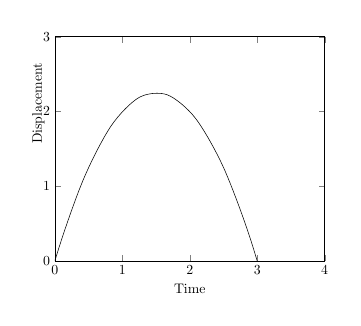
\begin{tikzpicture}[scale=0.5]
		\begin{axis}[xmin=0, ymin=0, xmax=4, ymax=3,
					 xlabel={Time}, xlabel style={below},
					 ylabel={Displacement}, ylabel style={right}]
			
			\addplot[mark=none, smooth] {-x^2+3*x};
		\end{axis}
	\end{tikzpicture}
	&
	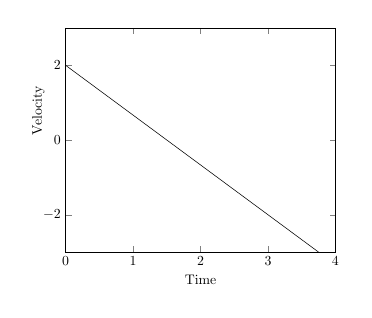
\begin{tikzpicture}[scale=0.5]
		\begin{axis}[xmin=0, ymin=-3, xmax=4, ymax=3,
					 xlabel={Time}, xlabel style={below},
					 ylabel={Velocity}, ylabel style={right}]
			
			\addplot[mark=none, smooth] {-(4/3)*x + 2};
		\end{axis}
	\end{tikzpicture}
	&
	\begin{tikzpicture}[scale=0.5]
		\begin{axis}[xmin=0, ymin=-3, xmax=4, ymax=3,
					 xlabel={Time}, xlabel style={below},
					 ylabel={Acceleration}, ylabel style={right}]
			
			\addplot[mark=none, smooth] {-2};
		\end{axis}
	\end{tikzpicture}
\end{tabular}
\caption{Graphs for a ball being thrown}
\end{figure}

We can see from this that when the displacement graph is a curve, the velocity is changing at a constant rate. If the velocity is a curve, acceleration is changing at a constant rate. The gradient of a displacement-time graph gives velocity, and the gradient of a velocity time graph gives acceleration. 

The reverse is also true: the area under the curve of an acceleration-time graph gives velocity, and the area under a velocity-time graph gives displacement. In calculus terms, the integral of acceleration with respect to time is velocity.

\subsection{Constant Acceleration Equations}

Motion with invariant acceleration can be described using a family of equations. Each of these use a combination of five variables:

\begin{itemize}
	\item $s$: displacement.
	\item $u$: initial velocity.
	\item $v$: final velocity.
	\item $a$: acceleration.
	\item $t$: time.
\end{itemize}

Each suvat equation uses four of these, meaning that all parameters can be calculated if we know only three.

\begin{definition}
	Suvat equations: $v=u+at$, $s=ut+\frac{1}{2}at^{2}$, $s=vt-\frac{1}{2}at^{2}$, $v^{2}=u^{2}+2as$, and $s=\frac{1}{2}(u+v)t$.
\end{definition}
We can combine, rearrange and evaluate these for different systems. It's important to note that sign is important. If you say that $a=-9.81$ then downward displacement should be negative.

\subsection{Projectile Motion}

Imagine a ball thrown horizontally from a height (maybe a cliff or a tower). It has some initial velocity $u$ and an initial height. The following is a diagram of the scenario.

\begin{figure}[ht]
\centering
	\begin{tikzpicture}
		\begin{axis}[xmin=-0.3, ymin=0, xmax=3, ymax=5, 
					 xticklabels={}, yticklabels={},
					 axis line style={draw=none}, tick style={draw=none},
					 smooth]
			
			%Trajectory
			\addplot[mark=none, red, very thick, domain=0:4] {-0.7*x^2+4};
			\addplot[mark=none, black, thick, domain=0:4] {0};
			
			%Nodes
			\node[circle, fill=black, minimum size=2mm, inner sep=0pt] (start) at (axis cs: 0,4){};
			\node (v) at (axis cs: 1.2,4){};
			\node (h) at (axis cs: 0,0){};
			\node[label=above:$v$] (v_label) at (axis cs: 0.6,4) {};
			\node[label=left:$s_{y}$] (h_label) at (axis cs: 0,2) {};
			
			%Draw
			\draw[-stealth, thick] (start) -- (v);
			\draw[|-|, thick] (start) -- (h.center);
		\end{axis}
	\end{tikzpicture}
	\caption{A ball is thrown with a horizontal velocity $v$ from a height $s_{y}$.}
\end{figure}

The time that the ball is in the air is, counter-intuitively, solely dependent on $s_{y}$ and on $a$, the acceleration. The time that it will take the ball to hit the ground is calculated as follows:
\[s_{y}=ut+\frac{1}{2}at^{2} \Rightarrow t=\sqrt{\frac{2s_{y}}{a}}\]
And the horizontal distance to the point of impact with the ground is given by:
\[v=\frac{s}{t} \Rightarrow s=vt\]

Now, consider a different scenario. The ball is now projected from the ground, with an initial velocity $v$ at an angle $\theta$ from the horizontal.

\begin{figure}[ht]
\centering
	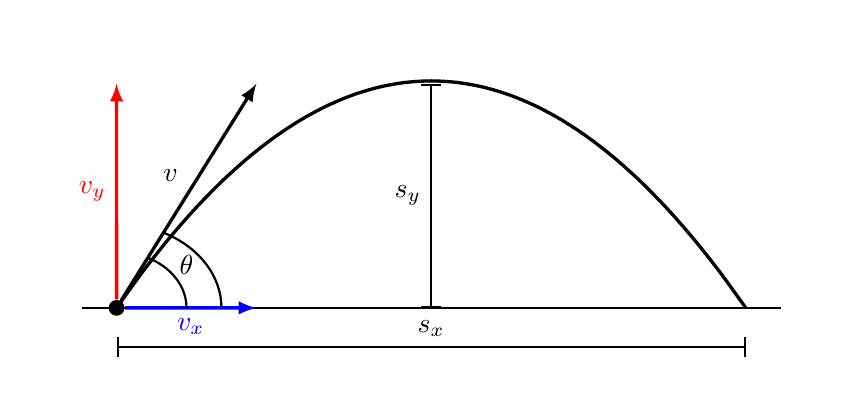
\begin{tikzpicture}
		\begin{axis}[xmin=-1, ymin=-1, xmax=10, ymax=5, yscale=0.5*1.5, xscale=0.95*1.5,
					 xticklabels={}, yticklabels={},
					 axis line style={draw=none}, tick style={draw=none},
					 smooth]
			
			%Trajectory
			\addplot[mark=none, black, very thick, domain=0:9] {-0.2*x^2+1.8*x};
			\addplot[mark=none, black, thick, domain=-0.5:9.5] {0};
			
			%Nodes
			\node[circle, fill=black, minimum size=2mm, inner sep=0pt] (start) at (axis cs: 0,0){};
			\node (max) at (axis cs: 4.5,4.05) {};
			\node[label=$\theta$] (angle_label) at (axis cs: 1,0.24) {};
			
			%Draw
			\draw[-latex, very thick] (start) -- (axis cs: 2,4) node [midway, above left] {$v$};
			\draw[-latex, very thick, blue] (start) -- (axis cs: 2,0) node [midway, below] {$v_{x}$};
			\draw[-latex, very thick, red] (start) -- (axis cs: 0,4) node [midway, left] {$v_{y}$};
			\draw[thick] (axis cs:1,0) arc (0:63:1);
			\draw[|-|, thick] (axis cs: 4.5,0) -- (axis cs: 4.5,4) node [midway, left] {$s_{y}$};
			\draw[|-|, thick] (axis cs: 0,-0.7) -- (axis cs: 9,-0.7) node [midway, above] {$s_{x}$};
			\draw[thick] (axis cs: 1.5,0) arc (0:63:1.5);
		\end{axis}
	\end{tikzpicture}
	\caption{A ball is thrown with a horizontal velocity $v$ at an angle $\theta$.}
\end{figure}

A fundamental principle is that the perpendicular components of velocity are independent of each other. The horizontal velocity $v_{x}$ is constant, and the vertical velocity $v_{y}$ is dependent on acceleration. This means that, again, time is solely dependent on $v_{y}$, and the horizontal distance on $v_{x}$. First, we need to resolve the velocity. Using trigonometry:
\[v_{x}=v\cos\theta\]
\[v_{y}=v\sin\theta\]
At the maximum of the curve, or the highest point, $v_{y}=0$. This makes sense, since it is the moment where the ball changes direction (and is when $\frac{ds}{dt}=0$). Knowing this fact, we can use $v^{2}=u^{2}+2as$ to calculate $s_{y}$:
\[v^{2}=u^{2}+2as \Rightarrow s_{y}=\frac{0-u^{2}}{2a}\]
Now that we know the maximum height, notice that the second half of this trajectory is identical to the scenario with horizontal motion. We can now use the same logic to find the time for the ball to drop from this point to the ground (i.e. the time for the second half of the trajectory)
\[s_{y}=ut+\frac{1}{2}at^{2} \Rightarrow t=\sqrt{\frac{2s_{y}}{a}}\]
Notice that when the start and end height are the same, the trajectory is symmeterical. This means that the time for the ball to reach the maximum point is the same as how long it takes for it to fall. Therefore, its total flight time is $2t$. Knowing this, we can calculate $s_{x}$. Horizontal velocity is constant so:
\[s_{x}=2tv_{x}\]

\section{Forces}

\subsection{The Newton}

\begin{definition}
	The newton ($\si{\newton}$, base units $\si{\kilo\gram\meter\per\second\squared}$) is the unit of force. One newton is the force required to give a mass of one kilogram an acceleration of one meter per second.
\end{definition}

The most fundamental equation of forces is derived from Newton's Second law of motion. It describes the simple relationship between the force an object feels, its mass and its acceleration.
\begin{equation}
	\sum\vec{F} = m \vec{a}
	\label{eq:newton}
\end{equation}
The force in this equation is the sum of the forces, or the net/resultant force on the object. This is shown in Figure \ref{fig:example}. In this case, the acceleration is felt in the direction of the net force. However, this does not mean that it is moving in this direction; the acceleration could be slowing it down, or changing it's direction of motion, we do not have the information necessary to determine what is the case.  

\begin{figure}[ht]
	\centering
	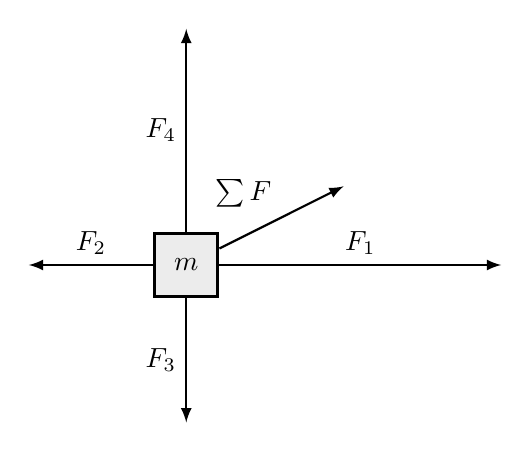
\begin{tikzpicture}
		%Node
		\node[rectangle, fill=gray!15, draw, minimum size=8mm, very thick] (obj) at (0,0) {$m$};
		
		%Vectors
		\draw[-latex, thick] (obj) -- (4, 0) node [midway, above] {$F_{1}$};
		\draw[-latex, thick] (obj) -- (-2,0) node [midway, above] {$F_{2}$};
		\draw[-latex, thick] (obj) -- (0,-2) node [midway, left] {$F_{3}$};
		\draw[-latex, thick] (obj) -- (0, 3) node [midway, left] {$F_{4}$};
		\draw[-latex, thick] (obj) -- (2, 1) node [midway, above left] {$\sum F$};
	\end{tikzpicture}
	\caption{Example free-body diagram}
	\label{fig:example}
\end{figure}

Newton's original second law defined the force as the rate of change in momentum with respect to time. We can simplify the differential to find Eq. \label{eq:newton}.
\[\vec{p}=m\vec{v} \text{ so } \sum\vec{F}=\frac{dm\vec{v}}{dt}\]
Factor out $m$:
\[\sum\vec{F}=m\frac{d\vec{v}}{dt} = m\vec{a}\]
by Definition \ref{def:accel}.

\subsection{Center of Mass}

The center of mass of an object is the point at which its mass appears to be concentrated. A force applied to this point causes the object to accelerate linearly. This means we also draw forces coming out of this point. The height of the center of mass is one of the two factors that determine the stability of an object. The other is the size of the base area. If the line of force passses through the base of the object, it will not topple. If it passes outside of this area it will fall over (Fig. \ref{fig:boxes}). Arc length is found by multiplying its corresponding angle by the radius. It so follows that the higher the center of mass is, the more unstable it is, since a smaller angle is capable of pushing the line of force outside of the base area.

\begin{figure}[ht]
\centering
	\begin{tabular}{c c}
		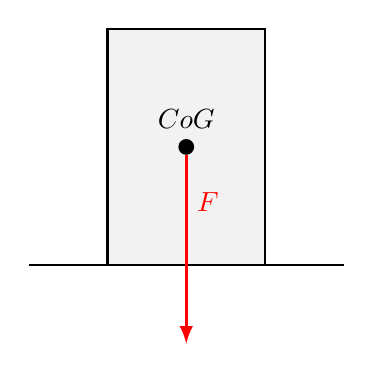
\begin{tikzpicture}
			\draw[thick] (-2,0)--(2,0);
			\draw[thick, fill=gray!10] (-1,0)--(1,0)--(1,3)--(-1,3)--(-1,0);
			\node[circle, fill=black, minimum size=2mm, inner sep=0pt, label=$CoG$] (cog) at (0,1.5){};
			\draw[-latex, very thick, red] (cog)--(0,-1) node [near start, right] {$F$};
		\end{tikzpicture}
		&
		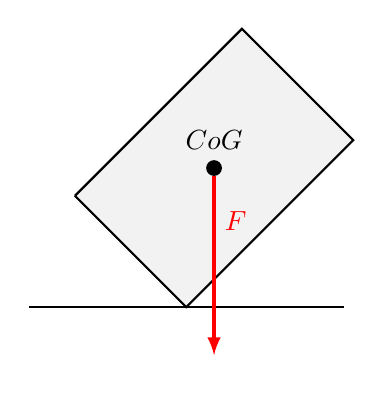
\begin{tikzpicture}
			\draw[thick] (-1,0)--(3,0);
			\begin{scope}[shift={({1-cos(45)},{sin(45)})}]
				\draw[thick, fill=gray!10, rotate=-45] (-1,0)--(1,0)--(1,3)--(-1,3)--(-1,0);
			\end{scope}
			\node[circle, fill=black, minimum size=2mm, inner sep=0pt, label=$CoG$] (cog) at (1+0.353,1.767){};
			\node[] (f) at (1+0.353,1.767-2.5){};
			\draw[-latex, very thick, red] (cog)--(f) node [near start, right] {$F$};
		\end{tikzpicture}
	\end{tabular}
	\caption{Boxes. The first is stable, the second is not.}
	\label{fig:boxes}
\end{figure}

